\documentclass[runningheads]{llncs}

\usepackage{amsmath}
\usepackage{amssymb}
\usepackage{booktabs}
\usepackage{array}
\usepackage{graphicx}
\usepackage{tikz}
\usetikzlibrary{arrows.meta, positioning, shapes.geometric, fit, calc}
\usepackage[hidelinks]{hyperref}
\hypersetup{colorlinks=false, pdfborder={0 0 0}}

\begin{document}

\title{Reproducible Detection of AI-Generated Faces via Open Handcrafted Features on PCA-Residual Images}

\author{[Author name]\inst{1} \and [Author name]\inst{1}}
\authorrunning{[Author et al.]}
\institute{[Department / University name] \\
\email{[email]}}

\maketitle

\begin{abstract}
Removing dominant principal components from a face image and inspecting the residual exposes differences between real photographs and AI-generated faces. A recent study demonstrated this effect through a Kolmogorov-Smirnov test using proprietary fractal descriptors, but the closed-source toolkit prevents independent replication, and no classifier was ever trained on the representation. We replace the proprietary descriptors with three open alternatives computed on the PCA residual of each 256$\times$256 grayscale face image: a 64-bin log-magnitude frequency histogram, a 59-bin rotation-invariant local binary pattern histogram, and a 64-bin Gaussian high-pass noise histogram. These are concatenated into a 187-dimensional feature vector. Five classical classifiers are evaluated on 40,000 balanced images drawn from FFHQ and a StyleGAN collection, split 80/10/10 with a fixed seed. The best-performing gradient-boosted tree reaches 86.9 percent accuracy and an area under the ROC curve of 0.944 on the held-out test set. A linear baseline already achieves 85.5 percent, suggesting that most of the separating signal resides in the descriptors themselves. The full pipeline uses only publicly available packages. We state which experiments remain open, including a sensitivity analysis of the truncation level and robustness testing under image perturbations.

\keywords{AI-generated face detection \and PCA residual \and handcrafted features \and local binary patterns \and frequency-domain analysis \and gradient boosting \and reproducibility}
\end{abstract}

\section{Introduction}

Synthetic face images have reached a quality that defeats casual human inspection. Generative adversarial networks, and more recently diffusion models, produce faces that look plausible at a glance. The detection community has responded mainly with deep neural networks trained directly on pixels. FaceForensics++~\cite{rossler2019} set the benchmark standard for this class of methods. Deep detectors work well in distribution, but they are expensive to train, and their internal logic is hard to examine. What feature drove a particular decision? The answer is distributed across millions of parameters.

A second, less fashionable line of work takes a different stance. Instead of learning features from data, it defines them by hand, computes a fixed-length vector for each image, and trains a simple classifier on that vector. The accuracy is usually lower. The trade-off is speed, interpretability, and the ability to point at a specific histogram bin and say what it measures. Recent studies by Yasir and Kim~\cite{yasir2025}, Nirob et al.~\cite{nirob2026}, and Chaudhari et al.~\cite{chaudhari2026} show that this approach remains active in 2025 and 2026, not a relic of an earlier era.

A separate thread of work, and the one most directly relevant here, concerns the input representation. Xie et al.~\cite{xie2026} proposed subtracting the dominant principal components from a face image and analyzing the residual. They showed, using fractal descriptors extracted with a proprietary toolkit called FreeAeon, that the distributions of these descriptors differ measurably between real and AI-generated faces. A Kolmogorov-Smirnov test confirmed the difference. Two things were missing. The toolkit is closed-source: nobody outside the authors can inspect how the fractal values are computed, and nobody can install the software to reproduce the experiment. And the analysis stopped at a statistical test. No classifier was trained. No accuracy was reported.

This leaves a gap. The PCA-residual representation has been shown to carry a signal, but the signal has never been used to build a detector that accepts an image and outputs a verdict.

We address both issues. First, we replace the closed-source descriptors with three alternatives that depend only on numpy, scikit-image, and OpenCV: a frequency-magnitude histogram, a local binary pattern histogram, and a noise-residual histogram. Second, we train five classical classifiers on the resulting 187-dimensional vector and report accuracy, F1, and AUC on a held-out test set. Third, we walk through every design choice in the pipeline at a level of detail sufficient for oral examination, so that each formula can be explained in plain language when questioned. Fourth, we name the experiments we did not run, a sensitivity sweep over the PCA truncation level, a controlled ablation comparing residual-based versus raw-image features, and robustness testing under compression and noise, rather than leaving these as implicit gaps.


\section{Related Work}

Detection methods for AI-generated faces fall broadly into two groups. One trains deep networks end to end on pixels. The other relies on handcrafted descriptors paired with classical machine learning.

In the first group, the benchmark established by R\"{o}ssler et al.~\cite{rossler2019} with FaceForensics++ remains the reference point. Xception-based pipelines reach high accuracy on the manipulations in that dataset, but the dataset focuses on face swaps and reenactments. Full-face GAN synthesis, the setting we address, is a different task. Numbers from FaceForensics++ cannot be compared directly with ours without retraining on the same data.

In the second group, three recent papers are closest to our work. Yasir and Kim~\cite{yasir2025} fuse HOG, LBP, and KAZE descriptors on raw face images and feed them to an ensemble of RandomForest, XGBoost, ExtraTrees, and SVC classifiers. They report 92 percent accuracy on FaceForensics++ and 96 percent on Celeb-DFv2. Nirob et al.~\cite{nirob2026} fuse a broader set of handcrafted descriptors, including color histograms, DCT, and wavelets, with a LightGBM classifier on the CIFAKE benchmark, reaching a PR-AUC of 0.988. Chaudhari et al.~\cite{chaudhari2026} combine HOG, LBP, and facial-landmark geometry with logistic regression, reporting around 90 percent on FaceForensics++. All three operate on raw images. None applies any form of residual preprocessing.

The frequency-domain half of our feature vector draws support from Zhang, Karaman, and Chang~\cite{zhang2019}, who showed that upsampling layers inside GAN generators leave structured artifacts in the frequency spectrum. Tan et al.~\cite{tan2024} built on this finding with FreqNet, a dedicated frequency-domain network presented at AAAI 2024, confirming that frequency information is a real and informative signal for deepfake detection. Our frequency histogram captures a coarser version of the same information without training a neural network.

The noise half draws on the Noiseprint work of Cozzolino and Verdoliva~\cite{cozzolino2018}, which demonstrated that camera and synthesis pipelines leave distinguishable noise fingerprints. Our Gaussian high-pass histogram is a much simpler extraction of the same intuition.

On the fractal side, the direct predecessor is Xie et al.~\cite{xie2026}, who introduced the PCA-residual representation and validated it with a distributional test using proprietary fractal descriptors. Xiao et al.~\cite{xiao2025} detect AI-generated images through fractal self-similarity in the frequency spectrum, a different mechanism that does not involve PCA residuals. Wang et al.~\cite{wang2025} use fractal structure for proactive watermark-based localization, a different problem entirely. Mohan and Peeples~\cite{mohan2024} show that lacunarity can be turned into a learnable pooling layer inside a neural network, pointing toward a path from fixed descriptors to trainable ones. Yang et al.~\cite{yang2016} used noise estimation and lacunarity for image tamper detection as early as 2016, predating the PCA-residual formulation by a decade. Giudice et al.~\cite{giudice2021} analyzed DCT statistics for GAN detection and tested robustness to JPEG compression. Hinke-Navarro et al.~\cite{hinke2025} fuse several handcrafted transforms with a deep RGB stream, representing the 2025 trend toward hybrid approaches.

Where does our paper sit? It takes the PCA-residual representation from~\cite{xie2026} and pairs it with the handcrafted-feature-plus-classical-ML recipe validated by~\cite{yasir2025},~\cite{nirob2026}, and~\cite{chaudhari2026} on raw images. No prior work we have found applies that recipe to PCA residuals. And no prior work in the PCA-residual line reports a classification accuracy. That is the gap this paper fills.


\section{Problem Formulation}

The task is binary classification. Given a single grayscale face image, decide whether it is a real photograph or an AI-generated face.

Let $I$ denote a grayscale image resized to 256 rows and 256 columns. We assign $y = 0$ to real images and $y = 1$ to generated ones. The classifier receives not $I$ itself but a feature vector $\phi(R) \in \mathbb{R}^{187}$, where $R$ is a residual image derived from $I$ by removing its dominant principal components, and $\phi$ is a fixed feature map that concatenates three histogram-based descriptors. The goal is to learn a function $f_\theta : \mathbb{R}^{187} \to [0,1]$ that estimates $P(y=1 \mid \phi(R))$ and thresholds it into a binary decision.

In plain terms: we strip away the large-scale structure of the face, extract three sets of statistics from what remains, and ask a classifier whether those statistics look more like a photograph or more like a generated image.


\section{Proposed Method}

\subsection{Pipeline Overview}

The pipeline has five stages, applied identically to every image regardless of whether it belongs to the training, validation, or test set (see Fig.~\ref{fig:pipeline}):
\begin{enumerate}[leftmargin=*]
    \item Load the image and convert it to grayscale at $256 \times 256$ resolution.
    \item Compute the PCA residual $R$, independently for that single image.
    \item Compute three histogram descriptors on $R$.
    \item Concatenate the three histograms into a 187-dimensional vector.
    \item Standardize each dimension to zero mean and unit variance using statistics from the training split only.
\end{enumerate}

Stage~5 is the only point where training-set statistics touch validation or test data, and they do so only through two numbers per dimension: a stored mean and a stored standard deviation.

\begin{figure}[t]
\centering
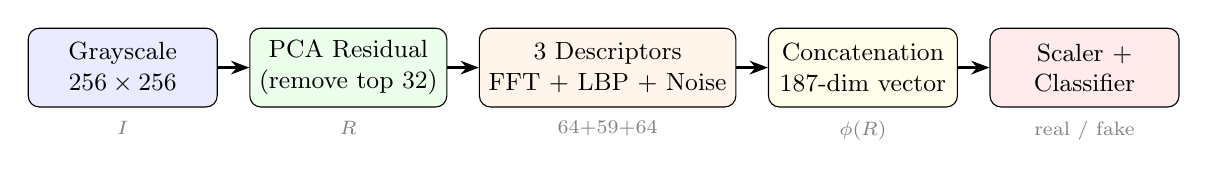
\begin{tikzpicture}[
    node distance=0.4cm,
    block/.style={rectangle, draw, rounded corners, minimum height=1.0cm, minimum width=2.4cm, align=center, font=\small},
    arrow/.style={-Stealth, thick},
    label/.style={font=\scriptsize, text=gray}
]
\node[block, fill=blue!8] (input) {Grayscale\\$256\times256$};
\node[block, fill=green!8, right=of input] (pca) {PCA Residual\\(remove top 32)};
\node[block, fill=orange!8, right=of pca] (feat) {3 Descriptors\\FFT + LBP + Noise};
\node[block, fill=yellow!8, right=of feat] (concat) {Concatenation\\187-dim vector};
\node[block, fill=red!8, right=of concat] (clf) {Scaler +\\Classifier};

\draw[arrow] (input) -- (pca);
\draw[arrow] (pca) -- (feat);
\draw[arrow] (feat) -- (concat);
\draw[arrow] (concat) -- (clf);

\node[label, below=0.05cm of input] {$I$};
\node[label, below=0.05cm of pca] {$R$};
\node[label, below=0.05cm of feat] {64+59+64};
\node[label, below=0.05cm of concat] {$\phi(R)$};
\node[label, below=0.05cm of clf] {real / fake};
\end{tikzpicture}
\caption{Pipeline overview. Each image passes through five stages: grayscale conversion, PCA-residual computation (removing the 32 dominant row-wise principal components), extraction of three histogram descriptors on the residual, concatenation into a 187-dimensional vector, and standardization followed by classification.}
\label{fig:pipeline}
\end{figure}


\subsection{PCA Residual Computation}

Each image is treated as a matrix of 256 row-vectors, each of length 256. Principal component analysis is fit on these 256 rows independently for that image alone. This produces an orthonormal basis $u_1, u_2, \ldots, u_{256}$ ordered by decreasing explained variance, and a row mean $\mu$.

Each row $I_i$ is projected onto this basis:
\begin{equation}
c_{i,k} = (I_i - \mu) \cdot u_k
\label{eq:projection}
\end{equation}

The residual image discards the projections along the top 32 directions and reconstructs each row from the remaining 224:
\begin{equation}
R_i = \mu + \sum_{k=33}^{256} c_{i,k}\, u_k = I_i - \sum_{k=1}^{32} c_{i,k}\, u_k
\label{eq:residual}
\end{equation}

\textit{What this means in plain language.} Every face image has large-scale structure: the overall brightness gradient, the rough shape of the face, the position of eyes and mouth. PCA captures these dominant patterns in its top components. When we throw those components away, what survives is fine-grained texture, subtle noise patterns, and small-scale irregularities. The hypothesis, first posed by Xie et al.~\cite{xie2026} and tested here with different descriptors, is that real cameras and AI generators leave different fingerprints in this fine-grained residual.

Why per-image PCA rather than a single global basis fit on the entire dataset? Because we care about the structure within each individual image, not about the variance across images. A global basis would mix inter-image variance (different faces) with intra-image structure (the texture of one face), and the residual would depend on which other images happened to be in the training set.

The truncation level $N = 32$ is inherited from the default used by Xie et al.~\cite{xie2026}. We did not sweep this parameter. Whether a different value of $N$ would raise or lower accuracy is an open question, stated explicitly in Sect.~\ref{sec:conclusion}.

% FIGURE 2 PLACEHOLDER
% \begin{figure}[t]
% \centering
% \includegraphics[width=\textwidth]{fig_pca_residual.png}
% \caption{PCA-residual visualization. Top row: four sample face images (two real from FFHQ, two generated by StyleGAN). Bottom row: the corresponding PCA residuals after removing 32 components. Residuals are contrast-enhanced for visibility. The dominant face structure has been removed; what remains is fine-grained texture where real and generated images are hypothesized to differ.}
% \label{fig:residual}
% \end{figure}


\subsection{Feature Extraction}

Three descriptors are computed on the residual image $R$, not on the original image $I$. Each one asks a different question about the residual.

\paragraph{Frequency descriptor (64 bins).} We compute the two-dimensional discrete Fourier transform of $R$, shift the zero frequency to the center, and take the logarithm of the magnitude:
\begin{equation}
m = \log(1 + |\mathcal{F}(R)|)
\label{eq:fft}
\end{equation}

The log transform compresses the dynamic range. Without it, a handful of large low-frequency coefficients would dominate the histogram, and the higher-frequency bins where generator artifacts tend to appear~\cite{zhang2019} would be drowned out. The 65,536 values of $m$ are binned into a 64-bin histogram spanning the image's own minimum and maximum log-magnitude, then normalized to sum to one.

\textit{What this descriptor captures.} GAN generators built from transposed convolutions and learned upsampling produce partially periodic patterns in the frequency domain~\cite{zhang2019, tan2024}. A histogram of log-magnitude values summarizes the overall frequency profile: how much energy sits at each scale, and whether the distribution looks like a natural photograph or something more regular.

\paragraph{Texture descriptor (59 bins).} A local binary pattern (LBP) is computed on $R$ with $P = 8$ sampling neighbors at radius $\rho = 1$, using the rotation-invariant variant \texttt{nri\_uniform} from scikit-image~\cite{ojala2002}.

For each pixel, LBP compares the pixel's value with its 8 neighbors, producing an 8-bit binary code. The \texttt{nri\_uniform} variant groups these codes into $P(P-1) + 3$ distinct categories. For $P = 8$, this gives $8 \times 7 + 3 = 59$ categories.

\textit{Why nri\_uniform and not uniform?} The simpler \texttt{uniform} variant produces only $P + 2 = 10$ distinct codes for $P = 8$. If you bin a 10-code output into a 59-bin histogram, 49 of the 59 bins will always be zero, regardless of image content. That wastes roughly a quarter of the 187-dimensional feature vector on structural zeros. The \texttt{nri\_uniform} variant fills all 59 bins.

\textit{What this descriptor captures.} LBP encodes micro-texture: the local pattern of brighter-than and darker-than relationships around each pixel. In the residual image, where large-scale face structure has been stripped away, these micro-patterns reflect fine texture produced by either the camera sensor or the generative model.

\paragraph{Noise descriptor (64 bins).} A Gaussian blur with a $5 \times 5$ kernel is applied to $R$, and the blurred image is subtracted from $R$ itself:
\begin{equation}
n = R - \mathrm{GaussianBlur}_{5 \times 5}(R)
\label{eq:noise}
\end{equation}

This is a high-pass filter. The result $n$ is a second-order residual: $R$ already removed the dominant PCA structure, and subtracting the blurred version of $R$ further removes its locally smooth content. What remains is pixel-level variation at the finest scale. The values of $n$ are binned into a 64-bin histogram over the fixed range $[-50, 50]$ and normalized to sum to one.

\textit{What this descriptor captures.} Camera sensors produce noise with particular statistical properties. AI generators produce a different kind of fine-grained variation. Cozzolino and Verdoliva~\cite{cozzolino2018} showed that these noise-level fingerprints can distinguish image sources. Our histogram is a much coarser version of the same idea.

\paragraph{Concatenation.} The three histograms are concatenated in fixed order (frequency, then texture, then noise), giving a $64 + 59 + 64 = 187$-dimensional raw feature vector.


\subsection{Feature-Extraction Algorithm}

\begin{table}[t]
\caption*{\textbf{Algorithm 1} \ PCA-Residual Handcrafted Feature Extraction}
\small
\begin{tabular}{@{}r@{\quad}l@{}}
\toprule
\multicolumn{2}{@{}l}{\textit{Input:} grayscale image $I$ of size $256\times 256$; $N=32$; $P=8$, $\rho=1$, method = nri\_uniform} \\
\multicolumn{2}{@{}l}{\textit{Output:} standardized feature vector $\phi(I) \in \mathbb{R}^{187}$} \\
\midrule
1: & Fit PCA on the 256 rows of $I$ $\to$ row mean $\mu$, directions $u_1, \ldots, u_{256}$ \\
2: & For each row $I_i$: $c_{i,k} = (I_i - \mu) \cdot u_k$ \\
3: & Zero out $c_{i,k}$ for $k = 1, \ldots, N$ (discard dominant directions) \\
4: & $R \leftarrow$ reconstruct from remaining coefficients (the PCA residual) \\
5: & $m \leftarrow \log(1 + |\mathrm{FFT2D}(R)|)$, zero-frequency centered \\
6: & $h_{\text{freq}} \leftarrow$ normalized 64-bin histogram of $m$ over $[\min(m), \max(m)]$ \\
7: & $L \leftarrow \mathrm{LBP}(R, P, \rho, \text{nri\_uniform})$ \\
8: & $h_{\text{tex}} \leftarrow$ normalized 59-bin histogram of $L$ over $[0, 59)$ \\
9: & $n \leftarrow R - \mathrm{GaussianBlur}_{5\times5}(R)$ \\
10: & $h_{\text{noise}} \leftarrow$ normalized 64-bin histogram of $n$ over $[-50, 50]$ \\
11: & $v \leftarrow \mathrm{concat}(h_{\text{freq}}, h_{\text{tex}}, h_{\text{noise}})$ \hfill \textit{187-dim raw vector} \\
12: & $\phi(I) \leftarrow (v - \mu_{\text{train}}) / \sigma_{\text{train}}$ \hfill \textit{standardize using training stats} \\
13: & \textbf{return} $\phi(I)$ \\
\bottomrule
\end{tabular}
\end{table}

\textit{Line-by-line explanation for oral defense.} Lines~1--4 are the core idea. We fit PCA on the rows of a single image, not on the whole dataset, which means no information from other images can leak into the residual. We throw away the top 32 components and keep only what PCA could not compress efficiently. Lines~5--6 ask whether the frequency content of the residual looks natural. Lines~7--8 ask whether the micro-texture looks natural, using a variant that fills all 59 bins. Lines~9--10 ask whether the finest-scale noise looks natural. Lines~11--12 combine and standardize.


\subsection{Classifiers}

Five classifiers are trained on the same 187-dimensional standardized vector. No per-classifier feature engineering is applied. (1)~Thresholded linear regression, the simplest possible baseline. (2)~RandomForest, a bagged ensemble of independently grown decision trees. (3)~XGBoost, (4)~LightGBM, and (5)~CatBoost, three gradient-boosted tree implementations that differ mainly in how they grow trees and regularize splits. All five use default hyperparameters. No hyperparameter search was performed.


\section{Experimental Setup}

\paragraph{Dataset.} 40,000 face images, balanced: 20,000 real from FFHQ~\cite{karras2019} and 20,000 AI-generated from the StyleGAN-based ``1 Million Fake Faces'' collection on Kaggle~\cite{tunguz2026}. Every image is converted to grayscale at $256 \times 256$ pixels.

\paragraph{Split.} 80/10/10 into training, validation, and test sets using stratified sampling with random seed 42. This gives 32,000 / 4,000 / 4,000 images, each split balanced.

\paragraph{Scaling.} StandardScaler fit on the 32,000 training vectors only, then applied unchanged to validation and test.

\paragraph{Model selection.} Validation confirms expected behavior. Each classifier is scored once on the test split. No hyperparameters were adjusted based on test scores.

\paragraph{Reproducibility.} The pipeline was executed end to end and independently rerun once. The two runs agreed within ordinary floating-point variation.


\section{Results and Discussion}

\subsection{Classification Performance}

Table~\ref{tab:results} shows the results. Every classifier beats the trivial 50 percent baseline by a wide margin.

\begin{table}[t]
\centering
\caption{Validation and test performance of all five classifiers on the 187-dimensional PCA-residual feature vector.}
\label{tab:results}
\small
\begin{tabular}{@{}lcccccc@{}}
\toprule
Classifier & Val Acc & Val F1 & Val AUC & Test Acc & Test F1 & Test AUC \\
\midrule
Linear regression (thr.)  & 0.8535 & 0.8556 & 0.9321 & 0.8552 & 0.8574 & 0.9309 \\
RandomForest              & 0.8355 & 0.8346 & 0.9121 & 0.8350 & 0.8338 & 0.9144 \\
XGBoost                   & 0.8680 & 0.8685 & 0.9415 & 0.8688 & 0.8687 & 0.9442 \\
LightGBM                  & 0.8690 & 0.8700 & 0.9424 & 0.8662 & 0.8664 & 0.9427 \\
CatBoost                  & 0.8602 & 0.8608 & 0.9360 & 0.8598 & 0.8594 & 0.9386 \\
\bottomrule
\end{tabular}
\end{table}

Validation and test numbers are close for every classifier, typically within half a percentage point of accuracy and within 0.003 of AUC. This consistency does not prove the absence of leakage, but it is what we would expect from a clean split.

% FIGURE 3 PLACEHOLDER
% \begin{figure}[t]
% \centering
% \includegraphics[width=0.7\textwidth]{fig_roc_curves.png}
% \caption{ROC curves for all five classifiers on the test set. XGBoost and LightGBM are nearly overlapping and closest to the top-left corner. RandomForest is the lowest.}
% \label{fig:roc}
% \end{figure}


\subsection{Which Classifier Family Wins}

XGBoost and LightGBM are essentially tied at the top. On the test set, XGBoost has the highest accuracy (0.8688), F1 (0.8687), and AUC (0.9442). LightGBM leads on all three validation metrics but falls slightly behind on test. The gap between them is around 0.002 to 0.003 on every metric, small enough that a different random seed could reverse it.

The more informative pattern is the gap between these two and RandomForest, which trails by roughly three accuracy points and 0.03 in AUC. All three are tree ensembles, but RandomForest grows trees independently and averages them, while the boosted methods grow trees sequentially, each correcting the errors of the previous. This suggests that the class-separating signal involves interactions among the three descriptor groups that sequential boosting exploits better than independent bagging.

% FIGURE 4 PLACEHOLDER
% \begin{figure}[t]
% \centering
% \includegraphics[width=0.7\textwidth]{fig_accuracy_bar.png}
% \caption{Test accuracy of all five classifiers. XGBoost and LightGBM are nearly equal and highest. The dashed line at 0.50 marks random guessing.}
% \label{fig:bar}
% \end{figure}


\subsection{The Linear Baseline Tells a Story}

The thresholded linear regression reaches 0.8552 test accuracy and 0.9309 AUC, within about one and a half percentage points of the best boosted tree. A purely linear decision boundary over 187 histogram bins already separates the two classes well. This means a large share of the real/fake signal is close to linearly separable. The gains from tree-based nonlinearity are a refinement of an already strong linear signal, not the source of most of the separability. We read this as evidence that the descriptors themselves, not the classifier, are doing most of the work.


\subsection{Caveats and Threats to Validity}

Several caveats bound what these numbers support.

The PCA truncation level $N = 32$ was inherited from~\cite{xie2026} and never swept. We do not know whether a different value would change accuracy.

We did not run a controlled ablation comparing the same descriptors extracted from the PCA residual against the same descriptors extracted from the raw image. The pipeline is motivated by the residual step, but this paper does not itself provide the single-variable comparison that would demonstrate the residual step's individual contribution.

No robustness test was performed. The numbers describe performance on clean images from the same acquisition and generation pipelines used at training time.

We did not fine-tune a deep baseline such as Xception on this exact split. The figures from~\cite{yasir2025} and~\cite{rossler2019} are cited as context, not as controlled comparisons.

The values in Table~\ref{tab:results} are point estimates from a single test split. We do not report confidence intervals.


\section{Conclusion}
\label{sec:conclusion}

This paper shows that the PCA-residual representation introduced by Xie et al.~\cite{xie2026} still separates real from AI-generated faces when paired with three open, publicly documented descriptors and a classical classifier, replacing the proprietary fractal descriptors used in the original study. On 40,000 balanced grayscale faces, gradient-boosted trees reach 86 to 87 percent accuracy and an AUC above 0.94. A linear classifier already reaches within roughly one and a half percentage points of that result, indicating that most of the separating signal lives in the descriptors rather than in classifier complexity.

Future work includes four extensions. First, a sensitivity sweep over the PCA truncation level $N$. Second, a controlled ablation comparing identical descriptors extracted from PCA residuals against those from raw images. Third, robustness testing under JPEG compression, blur, additive noise, and resizing, following~\cite{giudice2021}. Fourth, replacing fixed descriptors with a learnable formulation such as the lacunarity pooling layer proposed by~\cite{mohan2024}.


\begin{thebibliography}{17}

\bibitem{xie2026}
Xie, W., Yin, J., Ma, L., Zhang, X., Zhang, W.:
Fractal Characterization of Low-Correlation Signals in AI-Generated Image Detection.
arXiv:2604.17268 (2026)

\bibitem{xiao2025}
Xiao, S., Guo, Y., Peng, H., Liu, Z., Yang, L., Wang, Y.:
Generalizable AI-Generated Image Detection Based on Fractal Self-Similarity in the Spectrum.
arXiv:2503.08484 (2025)

\bibitem{rossler2019}
R\"{o}ssler, A., Cozzolino, D., Verdoliva, L., Riess, C., Thies, J., Nie{\ss}ner, M.:
FaceForensics++: Learning to Detect Manipulated Facial Images.
In: IEEE/CVF ICCV. arXiv:1901.08971 (2019)

\bibitem{yasir2025}
Yasir, M.A., Kim, H.:
Lightweight Deepfake Detection Based on Multi-Feature Fusion.
Applied Sciences \textbf{15}(4), 1954. arXiv:2502.11763 (2025)

\bibitem{wang2025}
Wang, T., Cheng, H., Liu, M.-H., Kankanhalli, M.:
FractalForensics: Proactive Deepfake Detection and Localization via Fractal Watermarks.
In: ACM Multimedia (Oral). arXiv:2504.09451 (2025)

\bibitem{mohan2024}
Mohan, S., Peeples, J.:
Lacunarity Pooling Layers for Plant Image Classification using Texture Analysis.
In: CVPR Workshops. arXiv:2404.16268 (2024)

\bibitem{zhang2019}
Zhang, X., Karaman, S., Chang, S.-F.:
Detecting and Simulating Artifacts in GAN Fake Images.
In: IEEE WIFS. arXiv:1907.06515 (2019)

\bibitem{hinke2025}
Hinke-Navarro, A., Nieto-Hidalgo, M., Espin, J.M., Tapia, J.E.:
Enhanced Deep Learning DeepFake Detection Integrating Handcrafted Features.
arXiv:2507.20608 (2025)

\bibitem{nirob2026}
Nirob, S.M.H., Rahman, M., Ehsan, S., Haque, S.:
Handcrafted Feature Fusion for Reliable Detection of AI-Generated Images.
arXiv:2601.19262 (2026)

\bibitem{chaudhari2026}
Chaudhari, L., Bansode, D., Patil, P., Magdum, S.:
DeepFake Face Detection with Handcrafted Features and Logistic Regression.
Int. J. Adv. Comput. Theory Eng. \textbf{15}(2S), 241--246 (2026)

\bibitem{yang2016}
Yang, Q., Peng, F., Li, J.-T., Long, M.:
Image Tamper Detection Based on Noise Estimation and Lacunarity Texture.
Multimedia Tools Appl. \textbf{75}(17), 10201--10211 (2016)

\bibitem{giudice2021}
Giudice, O., Guarnera, L., Battiato, S.:
Fighting Deepfakes by Detecting GAN DCT Anomalies.
J. Imaging \textbf{7}(8), 128 (2021)

\bibitem{cozzolino2018}
Cozzolino, D., Verdoliva, L.:
Noiseprint: A CNN-Based Camera Model Fingerprint.
arXiv:1808.08396 (2018)

\bibitem{tan2024}
Tan, C., Zhao, Y., Wei, S., Gu, G., Liu, P., Wei, Y.:
Frequency-Aware Deepfake Detection: Improving Generalizability through Frequency Space Learning.
In: AAAI. arXiv:2403.07240 (2024)

\bibitem{ojala2002}
Ojala, T., Pietik\"{a}inen, M., M\"{a}enp\"{a}\"{a}, T.:
Multiresolution Gray-Scale and Rotation Invariant Texture Classification with Local Binary Patterns.
IEEE Trans. PAMI \textbf{24}(7), 971--987 (2002)

\bibitem{karras2019}
Karras, T., Laine, S., Aila, T.:
A Style-Based Generator Architecture for Generative Adversarial Networks.
In: IEEE/CVF CVPR, pp. 4401--4410. arXiv:1812.04948 (2019)

\bibitem{tunguz2026}
Tunguz, B.:
1 Million Fake Faces. Kaggle dataset (2026)

\end{thebibliography}

\end{document}
